\chapter{Basic Statistics in Spreadsheets}

When you completed the problems in the last section, you probably noticed
how long it took to compute statistics like the mean, median,
and variance by hand. Luckily, computers were designed to free us from these
sorts of tedious tasks. The most basic tool for automating
calculations is the spreadsheet program.\index{spreadsheet}

The first spreadsheet program (VisiCalc) was introduced in 1979 as a
tool for finance people to play ``what if'' games.  For example, a
company might make a spreadsheet that told them how much more profit
they would make if they changed from using an expensive metal to using
a cheaper alloy.

There are lots of spreadsheet programs, including Microsoft's Excel, Google Sheets, and
Apple's Numbers. Any spreadsheet program will work; they are all very
similar. The instructions and screenshots here will be from Google
Sheets --- a free spreadsheet program you use through your web browser.

\section{The Barrel Problem}
In honor of this history, let's start by studying a business question:
You have a friend who dreams of quitting her job to become a cooper. (A
cooper makes barrels that are used for aging wine and whiskey.)  According to her:
\begin{itemize}
\item It costs \$45 dollars in materials to build one barrel.
\item A barrel sells for \$100 dollars.
\item The workshop/warehouse she wants to rent costs \$2000 per month.
\item Taxes take 20\% of her profits.
\item She needs to make \$4000 monthly after taxes.
\end{itemize}

She has asked you, ``How many barrels do I need to make each month?''


\section{Solving It Symbolically}

Many problems can be solved two ways: symbolically or
numerically.\index{symbolic vs. numeric solutions} To solve this
problem symbolically, you would write out the facts as equations or
inequalities, then do symbol manipulations until you ended up with
an answer. In this case, you would let $b$ be the number of barrels
and create the following inequality:

$$(1.0 - 0.2)\left(b(100 - 45) - 2000\right) \geq 4000$$

You would simplify it:

$$(0.8)\left(55 b - 2000\right) \geq 4000$$

And simplify it more:

$$44b - 1600 \geq 4000$$

If that is true, then:

$$44b \geq 5600$$

And if that is true, then:

$$b \geq \frac{1400}{11}$$

$1400/11$ is about 127.27, so she needs to make and sell 128 barrels
each month.

That is a perfect answer, and we didn't need a spreadsheet at all. However:
\begin{itemize}
\item As problems get larger and more realistic, it gets much more difficult to solve them symbolically.
\item As soon as you say ``Yes, you need to make and sell 128 barrels
  each month.'' Your friend will ask ``What if I make and sell 200
  barrels? How much money will I make then?''
\end{itemize}

So, we use a spreadsheets to solve the problem numerically.


\section{Your First Spreadsheet}

Let's first make an inital spreadsheet. 

In whatever spreadsheet program you are using, create a new spreadsheet document.

A spreadsheet is essentially a grid of cells. In each cell, you can put data (like numbers or text) and formulas.

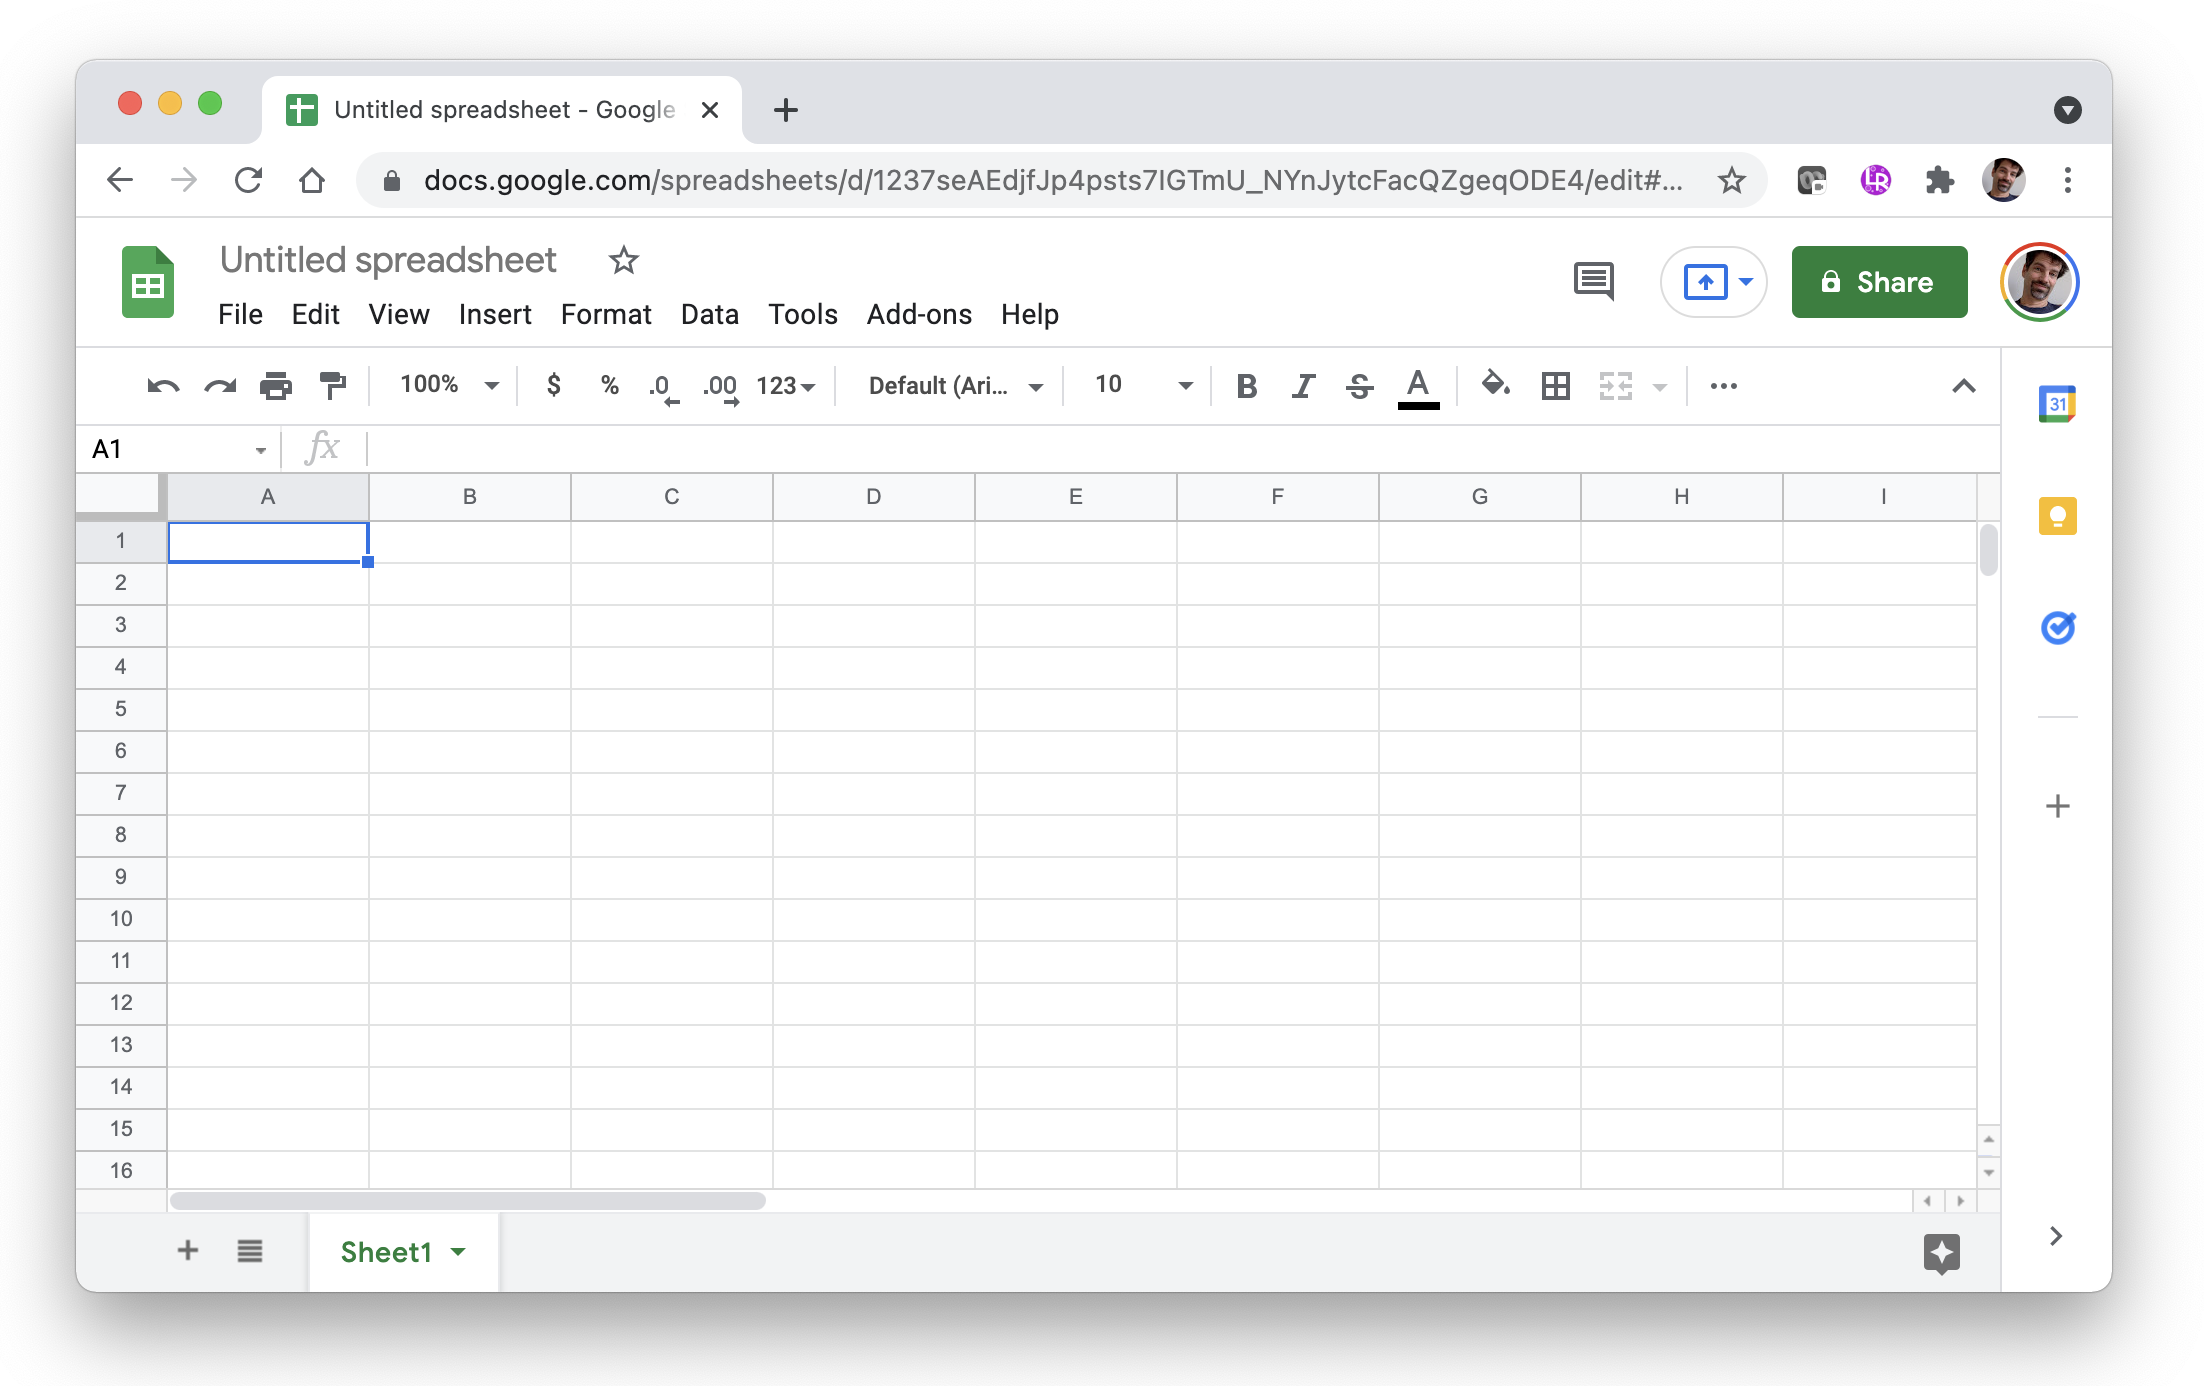
\includegraphics[width=0.6\textwidth]{BlankSheet.png}

Let's put some labels in the column:
\begin{itemize}
\item Select the first cell (A1) and type ``A number''.
\item Select the cell below it (A2) and type ``Another number''.
\item Select the cell below that one (A3) and type ``Their product''.
\item In the next column, type the number 5 in B1 and 7 in B2.
\end{itemize}

It should look like this:

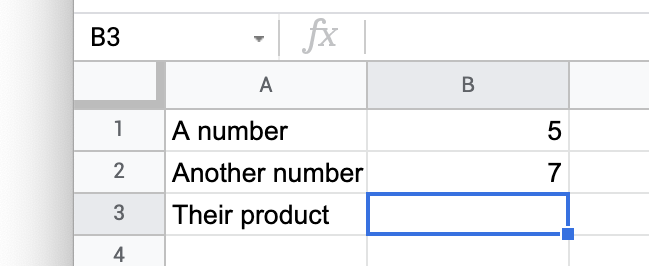
\includegraphics[width=0.5\textwidth]{NoFormulas.png}

Now, put a formula in cell B3. Select B3, and type ``= B1 * B2''. The spreadsheet knows this is a formula because it starts with `=`. It will look like this as you type:\index{Spreadsheet!Entering formula}

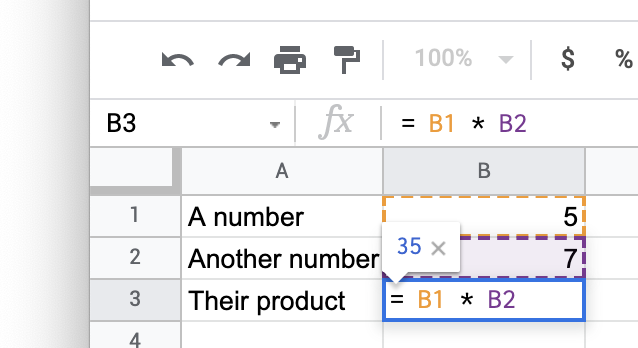
\includegraphics[width=0.5\textwidth]{TypingFirstFormula.png}

When you press Return or Tab, the spreadsheet will remember the formula, but display its value:

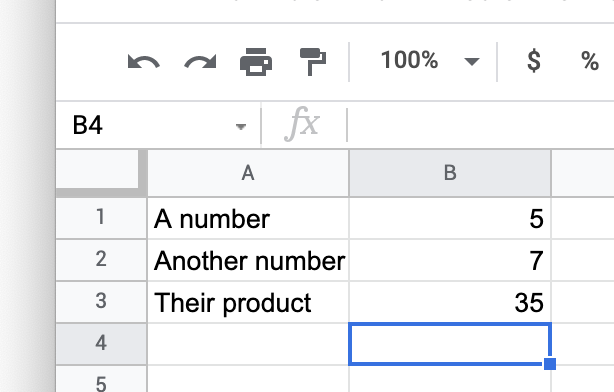
\includegraphics[width=0.5\textwidth]{FirstCalc.png}

If you change the values of cell B1 or B2, the cell B3 will automatically be recalculated. Try it.

\section{Formatting}

Every spreadsheet lets you change the formatting of your columns and cells. They are all a little different, so play with your spreadsheet a little now. Try to do the following:
\begin{itemize}
\item Set the background of the first column to light gray.
\item Right-justify the text in the first column.
\item Make the text in the first column bold.
\item Make the numbers in the second column have one digit after the decimal point.
\end{itemize}

It should look something like this:

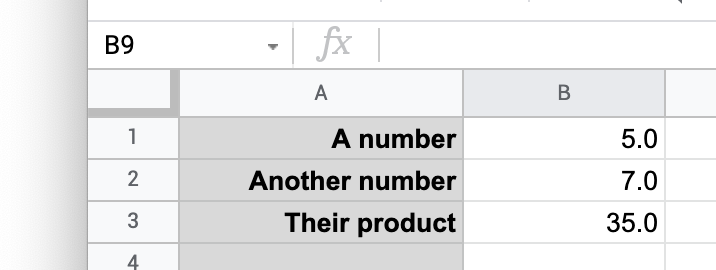
\includegraphics[width=0.6\textwidth]{FirstFormatting.png}

That's a spreadsheet. You have a grid of cells, each of which can hold a
value or a formula that uses values from other cells. The cells containing
formulas automatically update as you edit the values in the other
cells.

\section{Comma-Separated Values}

A large amount of data is exchanged in a file format called
\textit{Comma-Separated Values} or just CSV. Each CSV file holds one
table of data. It is a text file, and each line of text corresponds to
one row of data in the table. The data in each column is separated by
a comma. The first line of a CSV is usually the names of the
columns. A CSV might look like this:

\begin{Verbatim}
studentID,firstName,lastName,height,weight
1,Marvin,Sumner,260,45.3
2,Lucy,Harris,242,42.2
3,James,Boyd,261,44.2
\end{Verbatim}

In your digital resources for this module, you should have a file
called \path{1000cars.csv}. It is a CSV with only one column called
``speed''. The first few lines look like this:

\begin{Verbatim}
speed
33.8000
29.9920
34.8699
27.9936
\end{Verbatim}

There is a title line and 1000 data lines.

Import this CSV into your spreadsheet program. In Google Sheets, it looks like this:

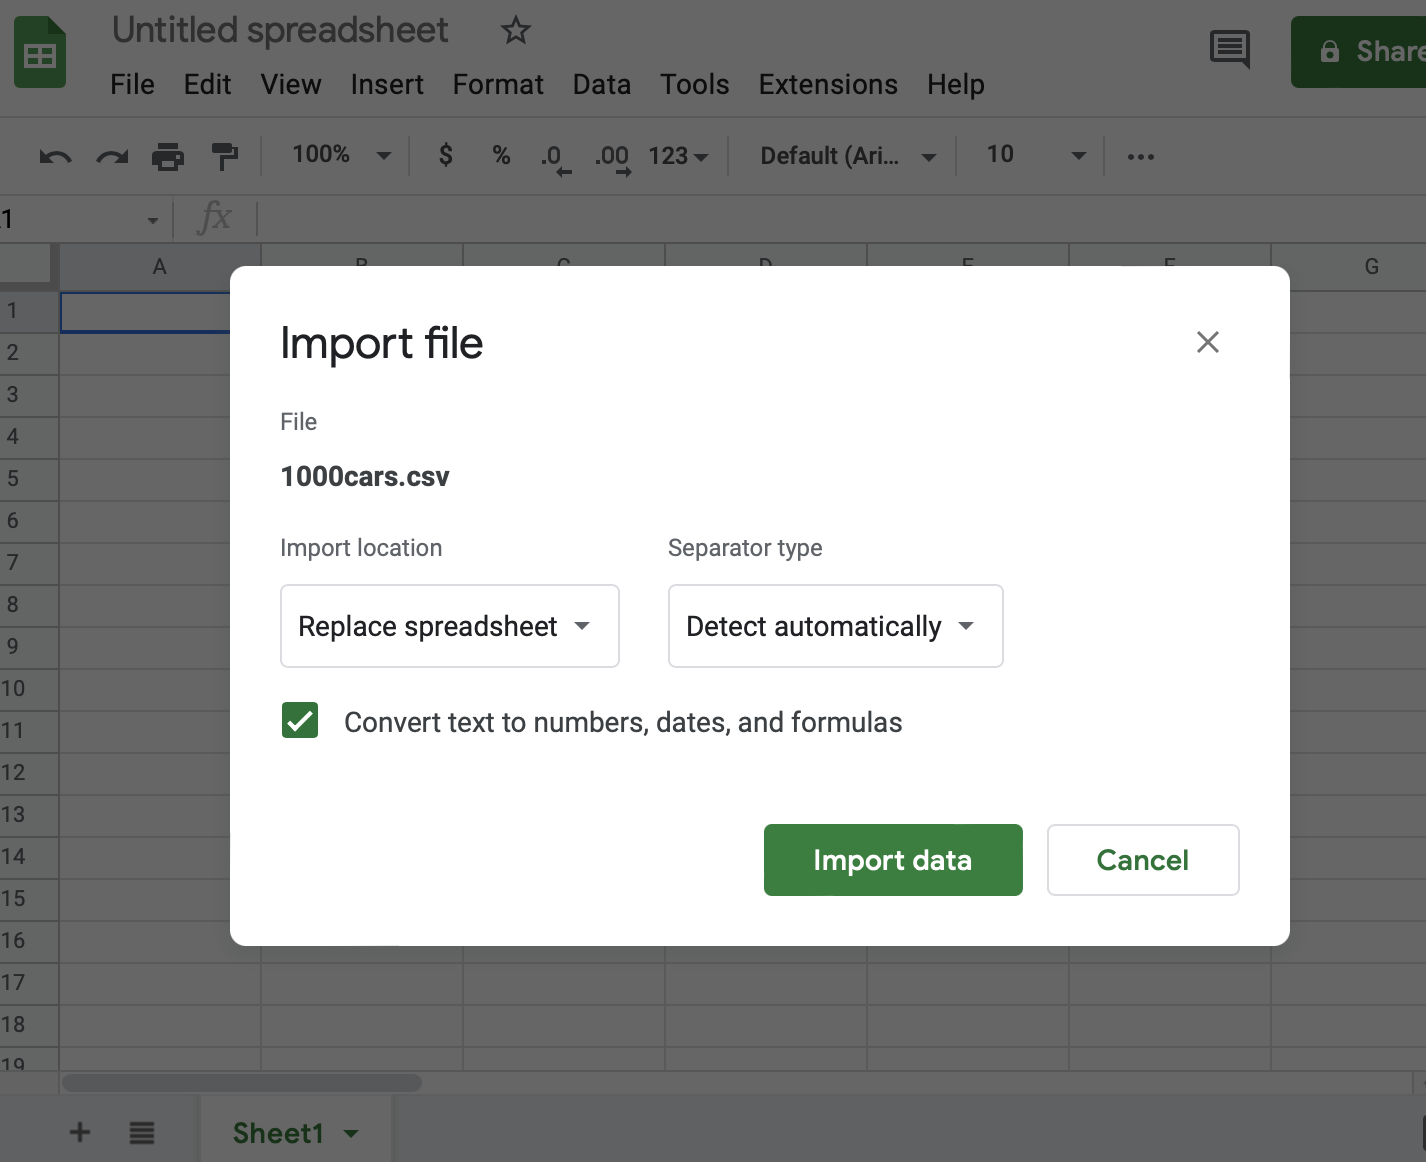
\includegraphics[width=0.5\textwidth]{ImportingCSV.png}

You should see a long, long column of data appear. (Mine goes from cell A2 through A1001.)

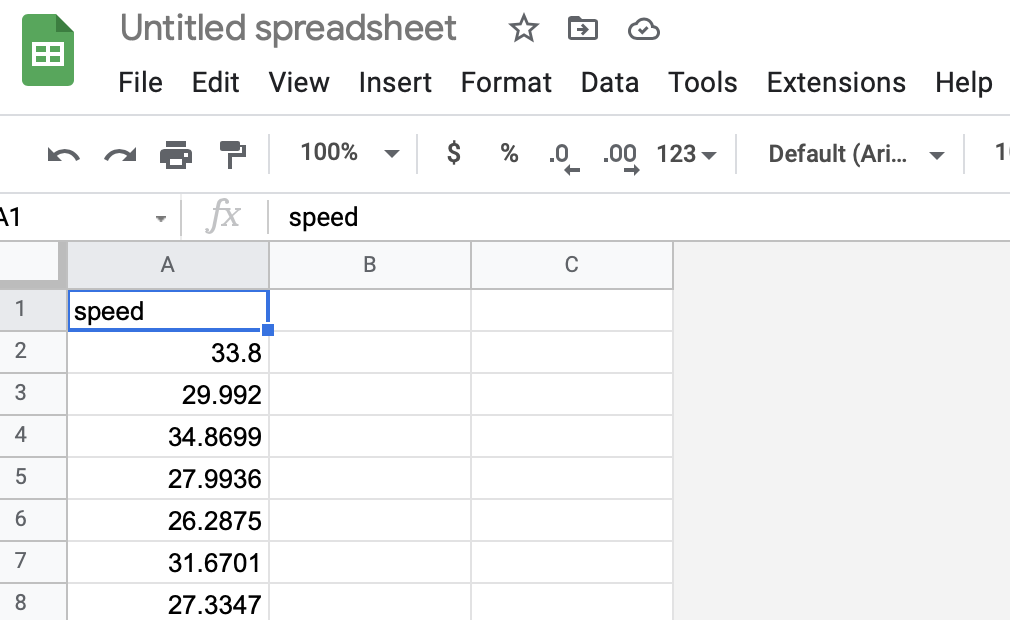
\includegraphics[width=0.5\textwidth]{ImportedCSV.png}

\section{Statistics in Spreadsheets}

Let's take the mean of all 1000 numbers.  In cell B2, type in a label:
``Mean''. (Feel free to format your labels as you wish. Bolding is recommended.)

In cell C2, enter the formula ``=AVERAGE(A2:A1001)''. When
you press return, the cell will show the mean: 31.70441, if done correctly.

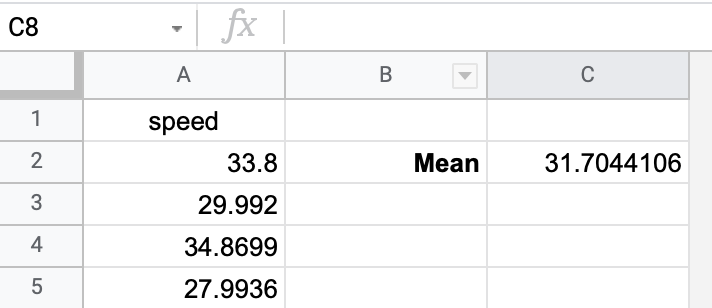
\includegraphics[width=0.4\textwidth]{Spread_mean.png}

Notice that by specifying that the function \pyfunction{AVERAGE} was to
be performed on a range of cells: cells A2 through (``:'') A1001.

Do the calculations for variance, standard deviation, and median.

\begin{itemize}
\item The function for variance is \pyfunction{VAR}.
\item The function for standard deviation is \pyfunction{STDEV}.
\item The function for median is \pyfunction{MEDIAN}.
\end{itemize}

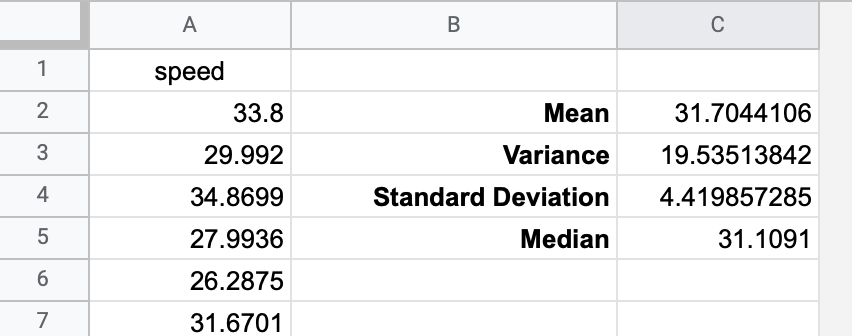
\includegraphics[width=0.4\textwidth]{var_stdev_median.png}

\section{Histogram}

Most spreadsheets have the ability to create a histogram. In Google
Sheets, you select the entire range A2:A1001 by selecting the first
cell and then shift-clicking the last. Next, you choose
Insert$\rightarrow$Chart. In the inspector, change the type of the
chart to a histogram (at the bottom under ``other''). This will get you a basic histogram.
% Add: Define histogram or give example, defined in basic statistics, must come previous

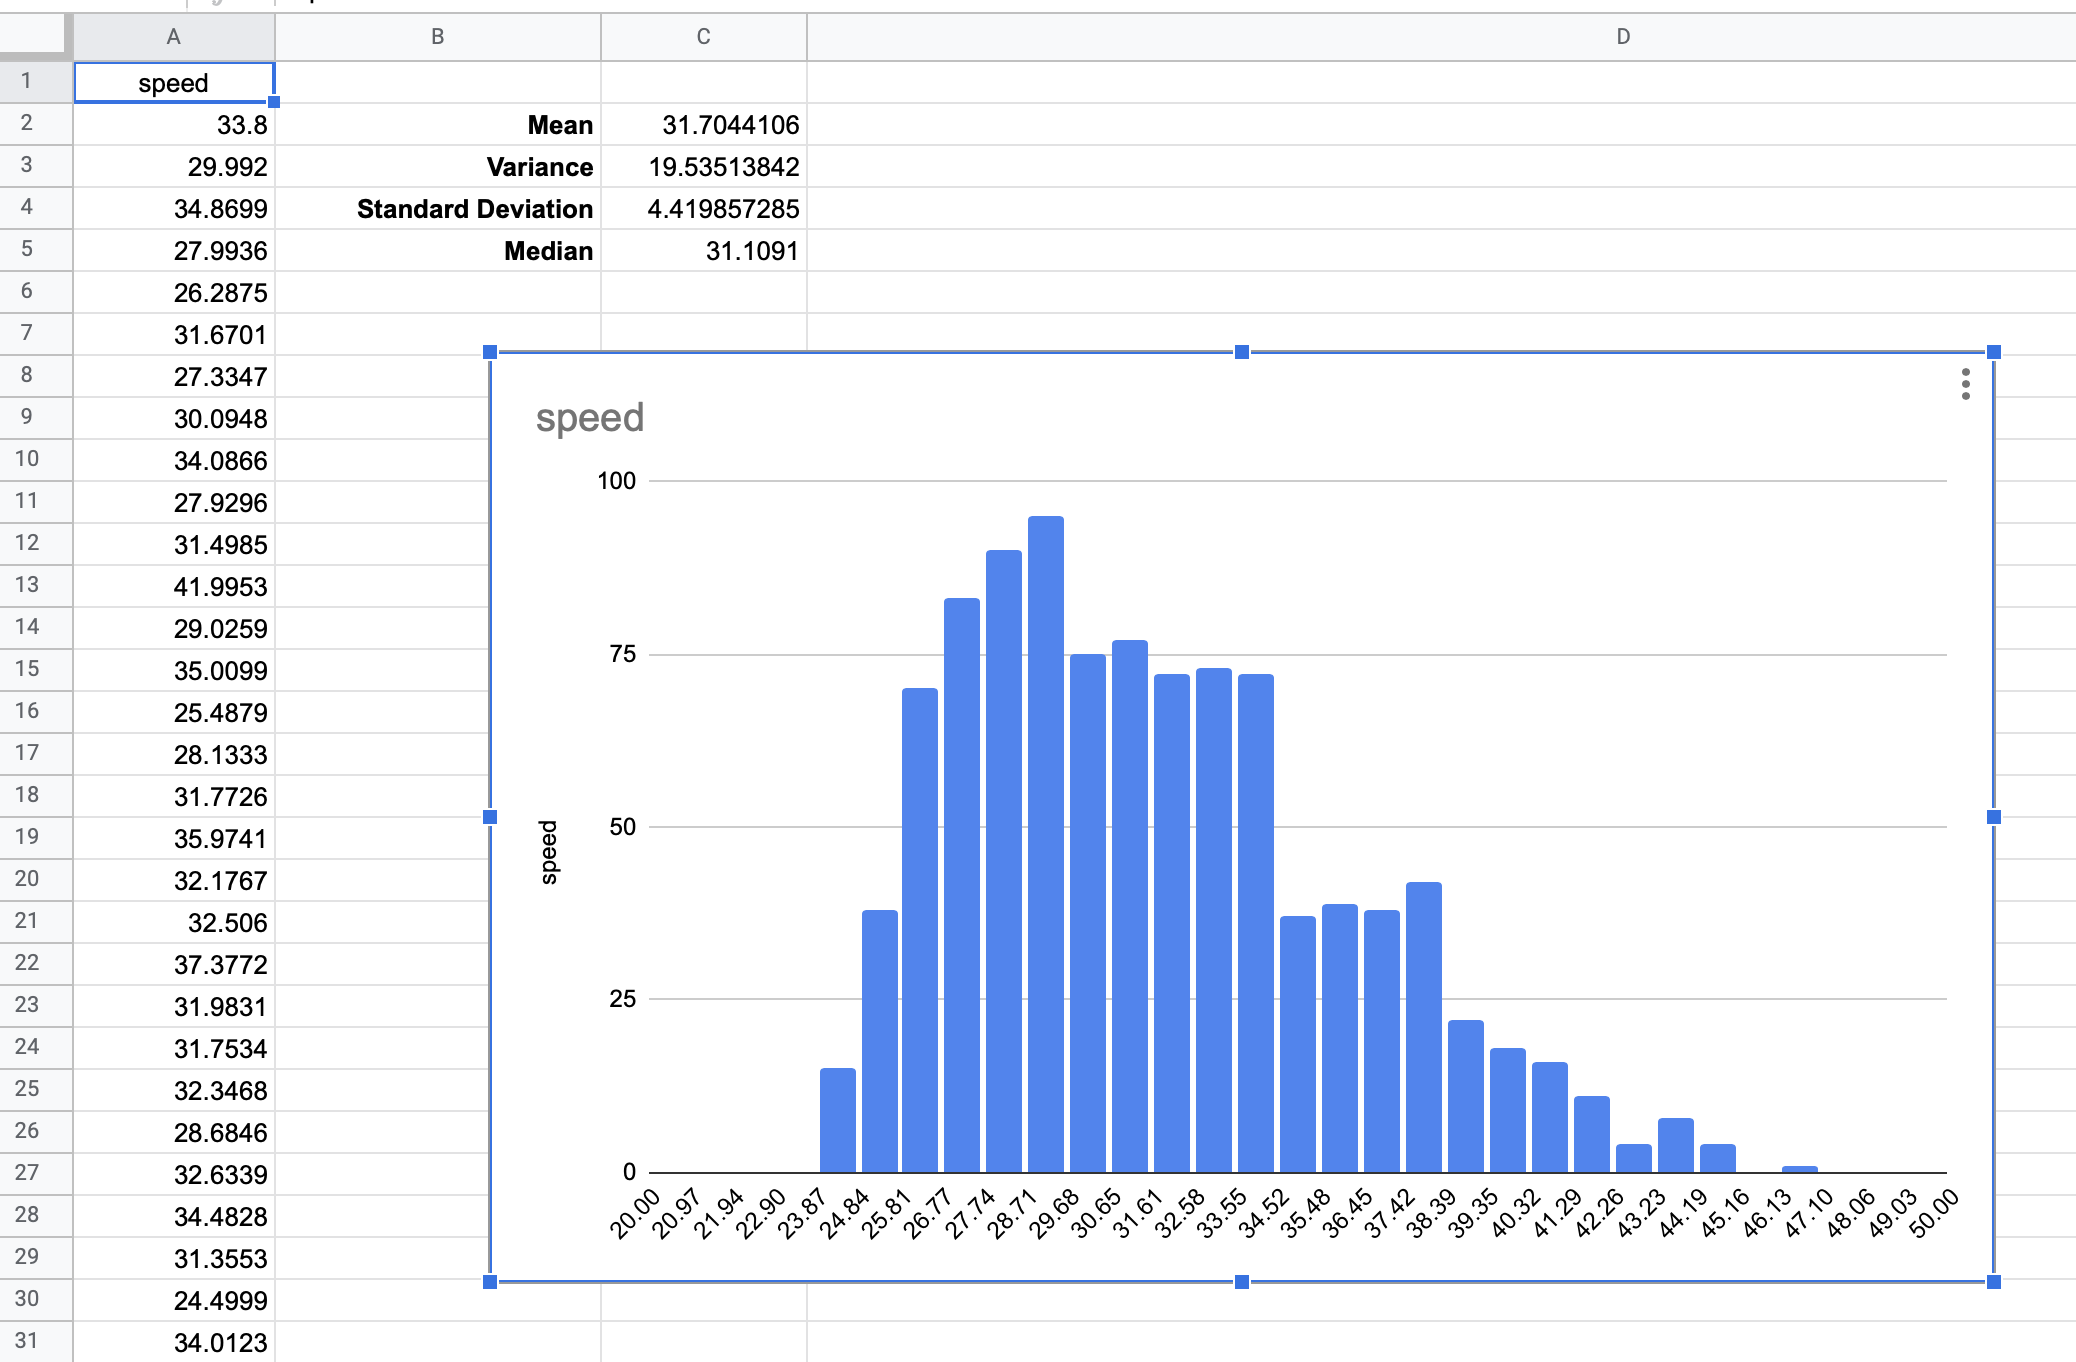
\includegraphics[width=0.7\textwidth]{default_histogram.png}

Play with the formatting to see how unique you can make data. Here is an example:

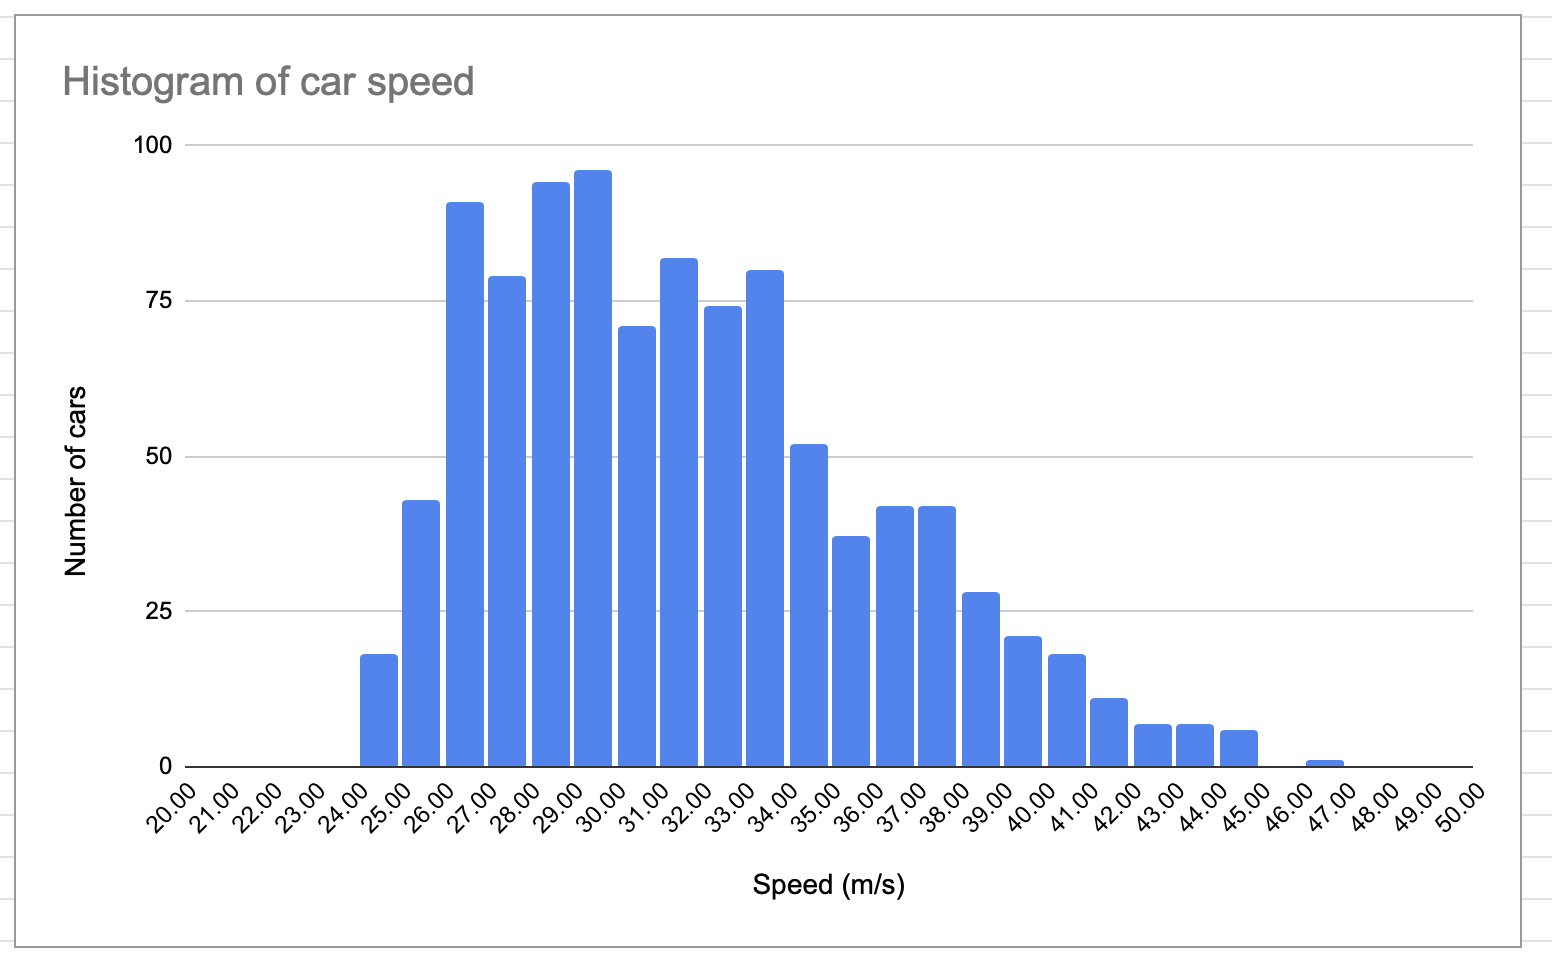
\includegraphics[width=0.8\textwidth]{final_histogram.png}

\begin{Exercise}[title={RMS}, label=rms_spreadsheet]

  In your spreadsheet, calculate the quadratic mean (the root-mean-squared) of the speeds.

  You will need the following three functions:
  \begin{itemize}
  \item \pyfunction{SUMSQ} returns the sum of the squares of a range of cells.
  \item \pyfunction{COUNT} returns the number of cells in a range that contains numbers.
  \item \pyfunction{SQRT} returns the square root of a number.
  \end{itemize}


\end{Exercise}
\begin{Answer}[ref=rms_spreadsheet]

The formula for the RMS is ``=SQRT(SUMSQ(A2:A1001)/COUNT(A2:A1001))''.
% KA: https://www.khanacademy.org/computing/ap-computer-science-principles/data-analysis-101/data-tools/a/learning-from-data-sets

\end{Answer}


\section{The Return of the Barrel Problem}

Let's get back to our example. Put labels in the A column:
\begin{itemize}
\item{Barrels produced (per month)}
\item{Materials cost (per barrel)}
\item{Sale price (per barrel)}
\item{Pre-tax earnings (per month)}
\item{Taxes (per month)}
\item{Take home pay (per month)}
\end{itemize}

Format them any way you like. It should look something like this:

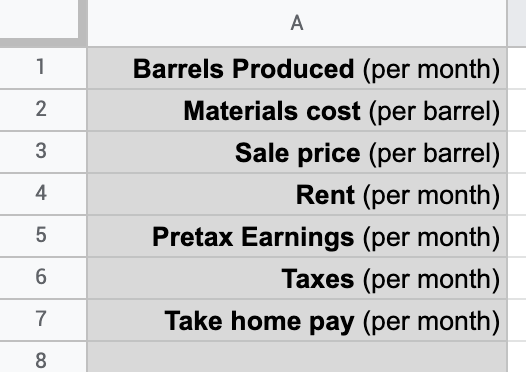
\includegraphics[width=0.4\textwidth]{BarrelLabels.png}

In the B column, the first four cells are values (not formulas):
\begin{itemize}
\item{115 formatted as a number with no decimal point}
\item{45 formatted as currency}
\item{100 formatted as currency}
\item{2000 formatted as currency}
\end{itemize}

It should look something like this:

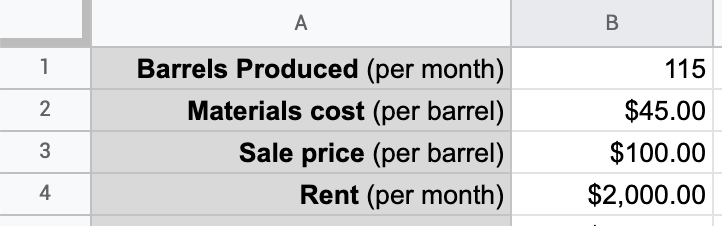
\includegraphics[width=0.5\textwidth]{BarrelValues.png}

The next three cells in the B column will have formulas:
\begin{itemize}
\item{B1 * (B3 - B2) - B4}
\item{0.2 * B5}
\item{B5 - B6}
\end{itemize}

It should look something like this:

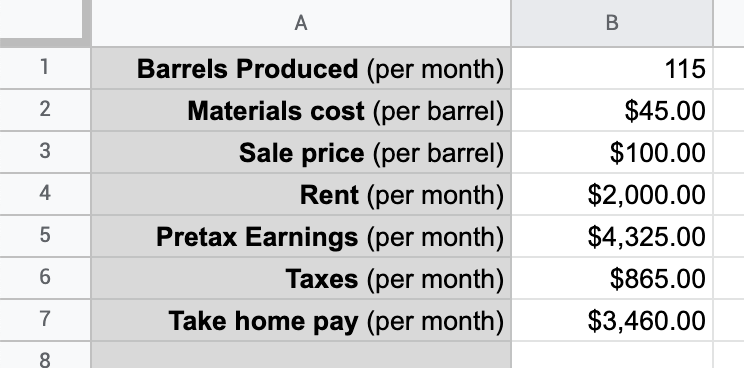
\includegraphics[width=0.5\textwidth]{BarrelFormulas.png}

Now you can share this spreadsheet with your friend, and she can put
different values into the cells for what-if games, such as ``If I can
get my materials cost down to \$42 per barrel, what happens to my take
home pay?''

Sometimes it is nice to show a range of values for a variable or two.
In this case, it might be nice to show your friend what the numbers
look like if she produces 115, 120, 125, 130, 135, or 140 barrels per
month.

We have one column, and now we need six. How do we duplicate cells?
\begin{enumerate}
\item Click B1 to select it, then shift-click on B7 to select all seven cells.
\item Copy them. (Depending on what program you are using, there is likely a menu item for this.)
\item Click C1 to select it
\item Paste them.
\end{enumerate}

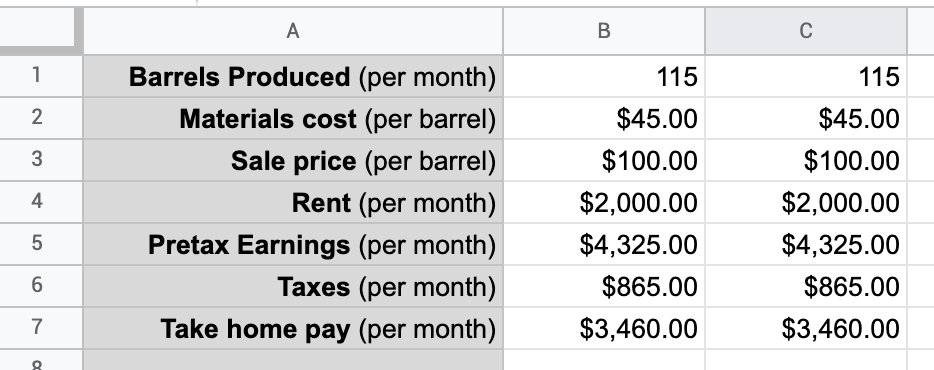
\includegraphics[width=0.5\textwidth]{BarrelCopyPaste.png}

We want the first cell in the new column to be 120. You could just
type in 120, but let's do something more clever. Put a formula into that
cell: = B1 + 5.  Now, the cell should show 120.

Why did we put in a formula? When we duplicate this column, this cell
will always have 5 more barrels than the cell to its left.

Next, let's duplicate the second column a few times. The easy way to do
this is to select the cells as you did before, then drag the lower-right
corner to the right until column G is in the selection. When you end
the drag, the copies will appear:

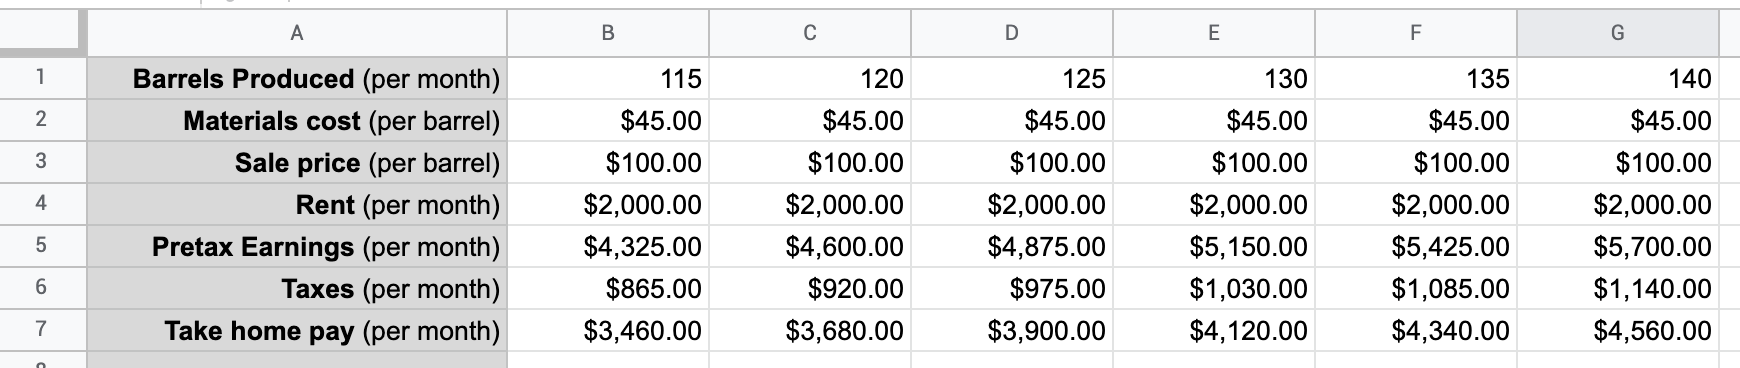
\includegraphics[width=0.8\textwidth]{BarrelDragPaste.png}

Nice, right? Now your friend can easily see how many barrels
correspond to how much take-home pay. But do you know what would be even more helpful? A graph.

\section{Graphing}

Graphing is a little different on every different platform.  Here is what you want the graph to look like:

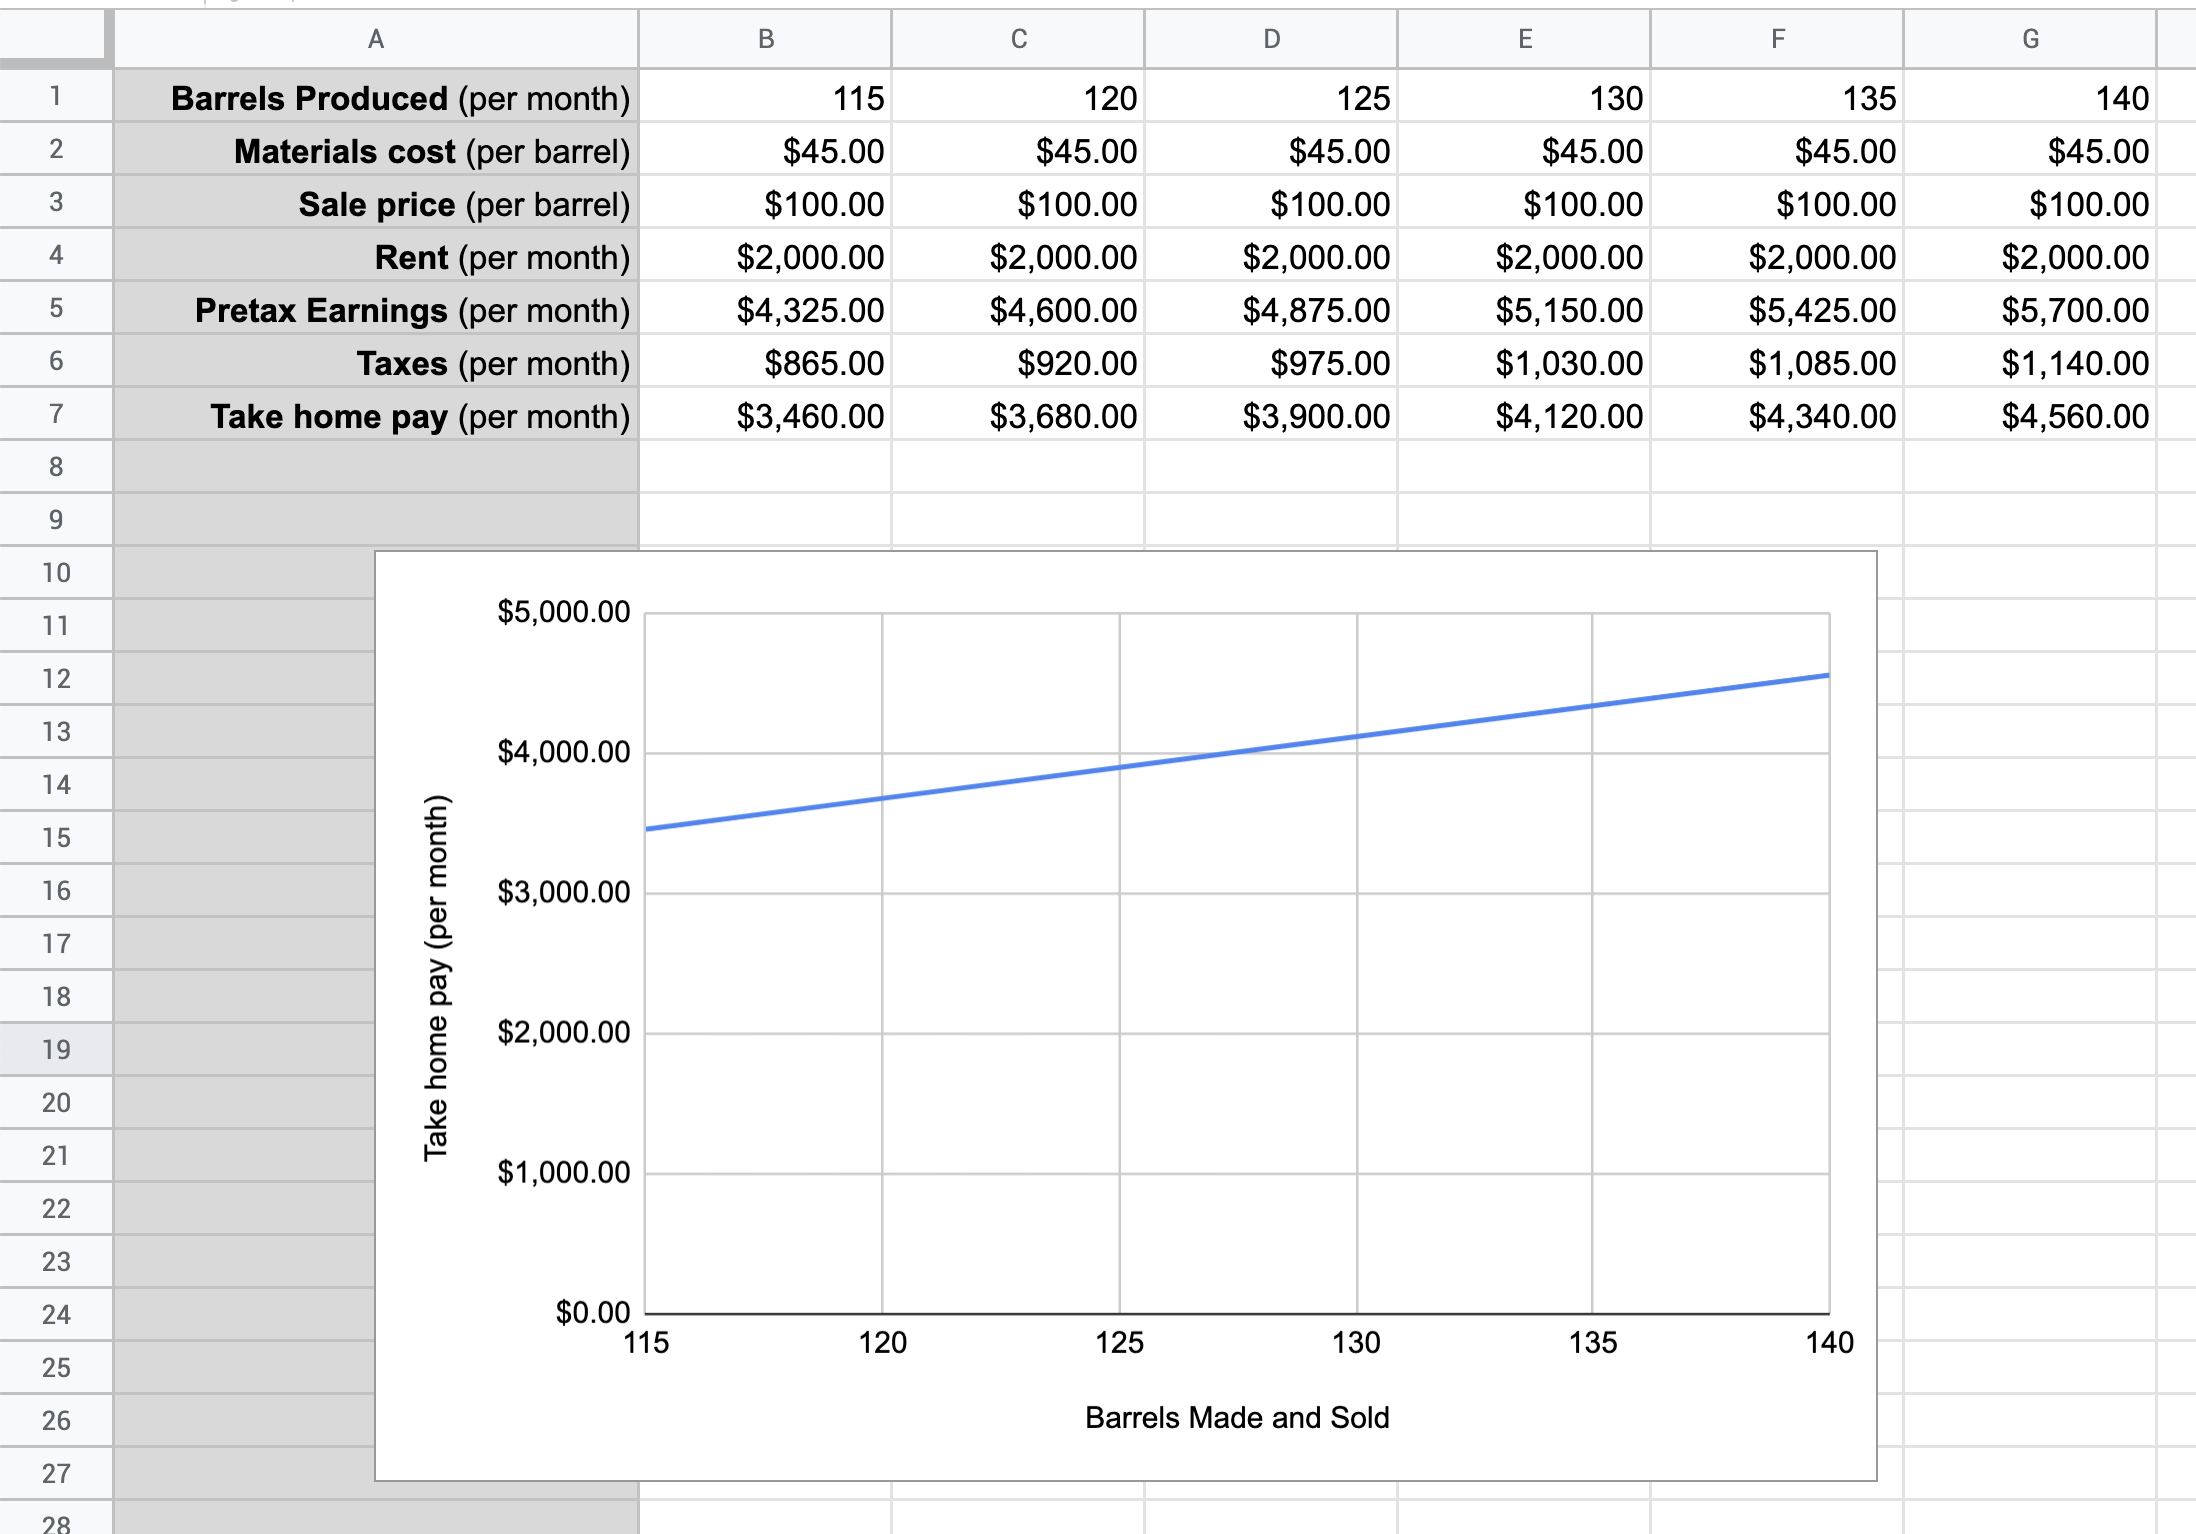
\includegraphics[width=0.8\textwidth]{BarrelGraph.png}

On Google Sheets:\index{spreadsheet!graphs}

\begin{enumerate}
\item Select cells B7 through G7. 
\item Choose the menu item Insert -> Chart.
\item Choose the chart type (Line)
\item Add the X-axis to be B1 through G1.
\item Under the Customize tab, Set the label for the X-axis to be ``Barrels Made and Sold''.
\item Delete the chart title (which is the same as the Y-axis label).
\end{enumerate}

\section{Other Things You Should Know About Spreadsheets}

Your spreadsheet document can have several ``Sheets''.  Each has its
own grid of cells.  The sheet has a name; usually, you call it
something like ``Salaries''.  When you need to use a value from the
``Salaries'' sheet in another sheet, you can specify ``Salaries!A2''
--- that is, cell A2 on sheet ``Salaries''.  To flip between the sheets,
there is usually a tab for each at the bottom of the document.

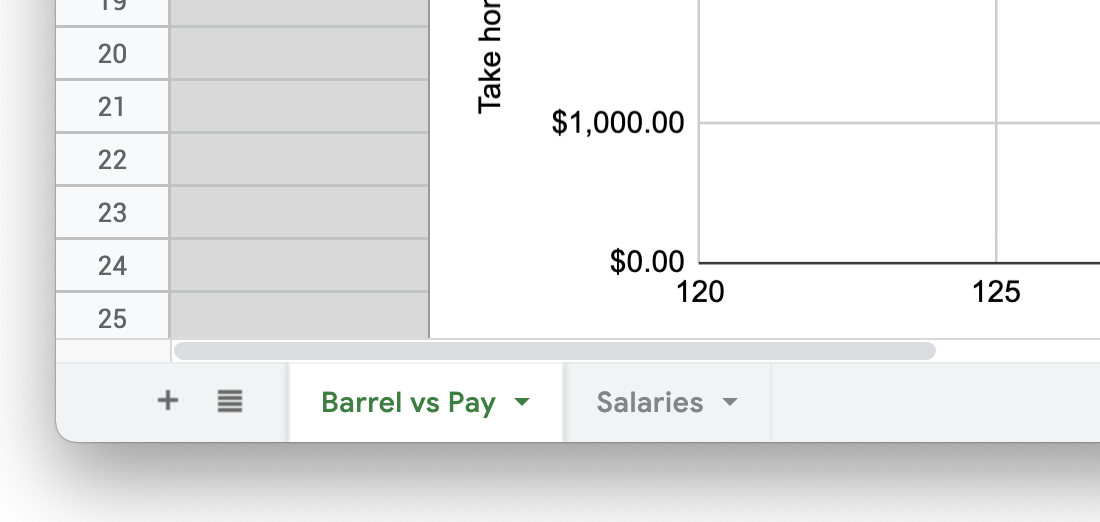
\includegraphics[width=0.5\textwidth]{Sheets.png}

By default, the cell references are relative. In other words, when you write
a formula in cell H5 that references the value in cell G4, the cell
remembers ``The cell that is one up and one to the left of me.''
Thus, if you copy that formula into B9, now that formula reads the
value from A8.

If you want an absolute reference, you use \$. If H5 references
\$G\$4, G4 will be used no matter where on the sheet the formula is
copied to.

You can use the \$ on the row or column. In \$A4, the column is
absolute and the row is relative.  In A\$4, the row is absolute and
the column is relative.

\section{Challenge: Make a spreadsheet}

You have a company that bids on painting jobs. Make a
spreadsheet to help you do bids. Here are the parameters:
\begin{itemize}
\item The client will tell you how many square meters of wall needs to be painted.
\item Paint costs \$0.02 per square meter of wall
\item On average, a square meter of wall takes 0.02 hours to paint.
\item You can hire painters at \$15 per hour.
\item You add 20\% to your estimated costs for a margin of error and profit.
\end{itemize}

Make a spreadsheet such that when you type in the square meters to be
painted, the spreadsheet tells you how much you will spend on paint
and labor.  It should also tell you what your bid should be.

